\chapter{Conclusie}
\label{cha:conclusie}
Het doel van dit rapport was het ontwerpen van een 'Pakkethondje' dat een gewicht van 10 kg over een hindernisbaan kan transporteren. De belangrijkste criteria bij dit ontwerp was het kunnen overnemen van een obstakel. 

\vspace{\baselineskip}
Tijdens het ontwerpproces zijn vier kansrijke ontwerpen ontwikkeld: de 'Mantis Car', de 'Uitschuiver', de 'Inklapper' en de 'Vierpoter'. Van deze ontwerpen zijn prototypes gemaakt die werden getest op de prestatiecriteria. Uit de testen bleek dat het meest kansrijke ontwerp een samenstelling is van de vier prototypes. Er is gekozen voor het mechanisme van de driepoot waarbij de schaarliften van de uitschuiver worden gebruikt. Dit eindontwerp gaat onder de naam 'Driepoter' en is te zien in \cref{fig:eindconcept}

\begin{wrapfigure}{r}{5.5cm}
    \centering
    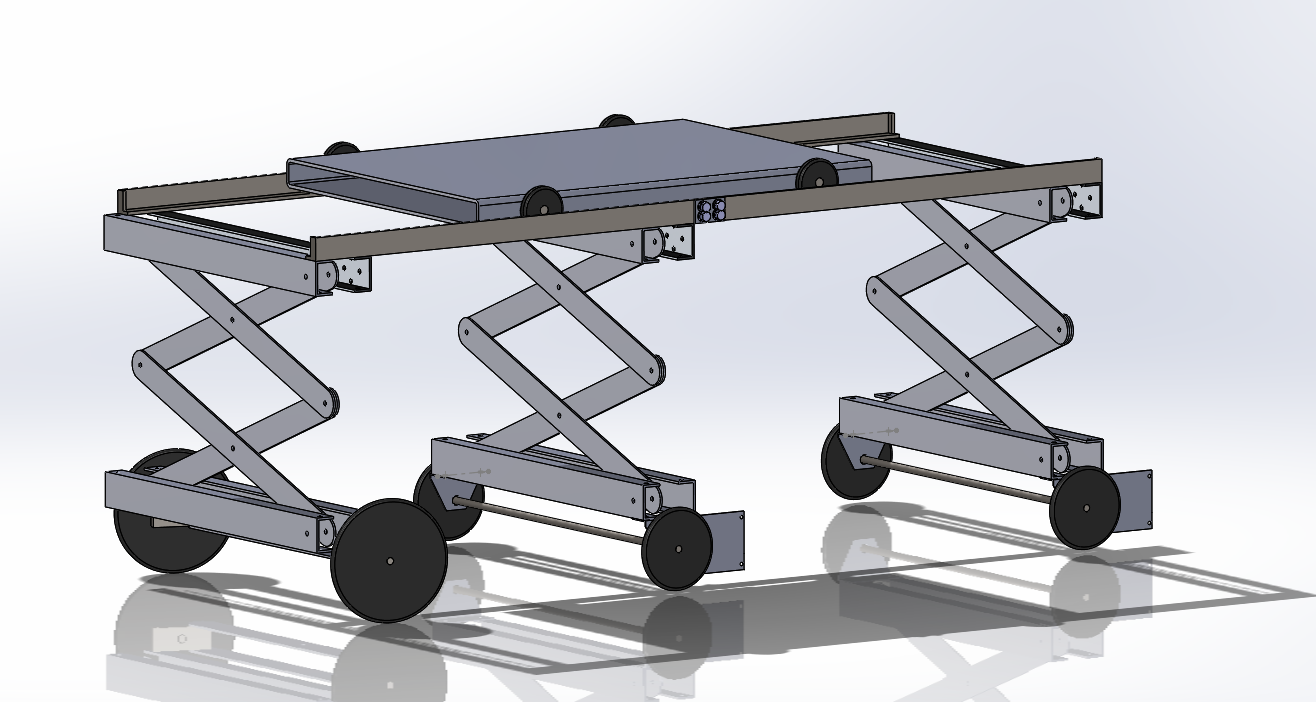
\includegraphics[width = 50mm]{05_conclusie/eindconcept.jpg}
    \caption{Solidworksmodel van het eindconcept}
    \label{fig:eindconcept}
\end{wrapfigure}

\vspace{\baselineskip}
De voornaamste reden voor het kiezen van de schaarlift is dat het stabieler is dan de andere deelontwerpen. Een tweede reden voor het kiezen van de schaarlift is in verband met de lengte van het voertuig. Het gebruik van inklapbare poten vereist een zeer lange kar, wat zorgt voor problemen tijdens het sturen.  Een andere reden voor de schaarlift is de veelzijdigheid van het ontwerp. Schaarliften kunnen gemakkelijk een verticale beweging opdoen, waardoor het over de meeste obstakels kan rijden. Deze eigenschap missen de andere concepten.

Hoewel de schaarlift de beste keuze blijkt te zijn, zijn er nog een aantal aanbevelingen voor volgende rapporten. Aanbeveling 1 is het onderzoeken van de schaarliften en of ze op de manier hoe ze in dit concept zijn geconstrueerd ook wel echt ideaal zijn. Misschien is er nog een betere versie van de schaarlift waardoor het eindconcept nog verder verbeterd zou kunnen worden. Aanbeveling 2 zou het onderzoeken van de duurzaamheid van het eindconcept kunnen zijn. Zijn er misschien betere motoren en/of materialen die de gevraagde functies vervullen en ook beter zijn voor het milieu zou een vraag kunnen zijn die kan volgen op dit rapport.



% Refereer naar de MCA!! Gewicht, kosten, snelheid, duurzaamheid, etc.
